% !TeX root = RJwrapper.tex
\title{corVis: An R Package for Visualising Associations and Conditional
Associations}
\author{by Amit Chinwan and Catherine Hurley}

\maketitle

\abstract{%
Correlation matrix displays are important tools to explore multivariate
datasets prior to modeling. These displays with other measures of
association can summarize interesting patterns to an analyst and assist
them in framing right questions while performing exploratory data
analysis. In this paper, we present new visualisation techniques to
visualise association between all the variable pairs in a dataset in a
single plot, which is something existing displays lack. We extend these
displays to regression and classification settings, where these could be
used to find out variables with high predictive power. Also, we propse
new methods to visualise trivariate relationship summaries using
conditioning. We use different layouts like: matrix or linear, to name a
few, for our displays which have their own advantages and disadvantages.
We use seriation in our displays which helps in highlighting interesting
patterns easily. The R package \emph{corVis} provides an implementation.
}

\hypertarget{section-1-introduction}{%
\section{Section 1: Introduction}\label{section-1-introduction}}

Exploratory Data Analysis (EDA) is an important step to explore
multivariate datasets prior to modeling. One of the important tools used
for EDA is correlation matrix display, also known as \emph{corrgram}
\citep{friendly2002corrgrams}. This display is produced by first
calculating the correlation among the variables and then plotting these
calculated values in a matrix display. Effective ordering techniques are
also used with these displays to highlight interesting relationships.
The display is useful to quickly find highly associated variables which
are explored further and are taken into consideration during the
modeling step.

The correlation displays are generally used with one of the Pearson's,
Spearman's or Kendall's correlation coefficient and are therefore
limited to quantitative variables. An analyst can use one-hot encoding
of the qualitative variables in order to use these displays but will
need to deal with the high dimensions produced by the encoding. The
existing method to quickly explore association among qualitative
variables, and mixed variables in a dataset include using proportions or
counts with different graphical displays like boxplots or barplots
depending on the variable types. This means that the analyst will have
to explore quantitative, qualitative and mixed variables separately and
thus calls for a tool which can summarize relationships among all the
variables in a single step.

MANY ASSOCIATION measures have been proposed to summarize different
types of relationships among two variables. The most commonly used
measure is Pearson's correlation coefficient which captures any linear
trend present between the variables. Other popular measures include
Kendall's or Spearman's rank correlation coefficient which are
non-parametric measures and looks for monotonic relationship among the
variables. The distance correlation \citep{szekely2007measuring} is an
important measure useful in exploring non-linear relationships. The
information theory measure maximal information coefficient
\citep{reshef2011detecting} is capable of summarizing complex
relationships. These multiple measures are useful for explaining complex
relationships in a dataset compared to using a single measure. With
effective displaying techniques, the multiple measures of association
provide a comparison tool that assist an analyst in discovering
interesting variable pairs.

The association measures calculated at different levels of a factor
variable for a variable pair help in finding patterns like Simpson's
paradox and displaying these conditional associations using graphical
representation will help explain these patterns.

In this paper, we propose extensions of these displays and new
visualizations which look at variables of mixed type, multiple
association measures and conditional associations. These displays are
implemented in the R package \texttt{corVis}. The paper is organised in
the following way: first a review of existing packages/methods to
calculate and display association with a quick overiew of some
association measures used in the package, then our approach to calculate
the association measures, then visualizations of associations and
conditional associations, followed by a discussion.

\hypertarget{section-2-background}{%
\section{Section 2: Background}\label{section-2-background}}

The correlation matrix display is an important tool to explore
association among variables in a multivariate analysis. It was first
introduced by \citet{murdoch1996graphical} in which they replaced the
numerical entries of a correlation matrix with ellipses and then
popularized by \citep{friendly2002corrgrams} who called them
\emph{corrgrams}, wherein he rendered the correlation values with shaded
squares, bars, ellipses, or circular `pac-man' symbols. The main goal of
these displays is to describe the bivariate patterns in a dataset. This
section provides a brief review of correlation displays and the
association measures which are used to explore interesting
relationships.

\hypertarget{section-2.1-literature-review-on-correlation-displays}{%
\subsection{Section 2.1: Literature Review on Correlation
Displays}\label{section-2.1-literature-review-on-correlation-displays}}

There are packages available in R which can be used to create
correlation matrix displays. The R package \CRANpkg{corrgram} provides
these displays with shaded squares, bars, ellipses, or circular
`pac-man' glyphs. The package includes various variable ordering methods
which assist in detecting patterns of relations among the variables. The
package \CRANpkg{corrr} produces correlation matrix in a \texttt{tidy}
structure, which then can be used to create correlation displays. In
addition to matrix display, the package also plots the correlation
values in a network display which is useful when dealing with
high-dimensional datasets. There have been other extensions to
correlation displays like: \citep{buja2016visualization} and
\CRANpkg{sCorrPlot}, which have been proposed mainly for exploring
correlations among the numeric variables for a high dimensional dataset.
We introduce a display which includes all the variables of a dataset,
irrespective of the data type, displaying every pairwise association.
This saves the effort and time of an analyst for exploring relationship
among all the variable pairs. \citet{kuhn2013applied} have proposed
display techniques to compare multiple association measures for every
pair of output variable and a predictor to measure the importance of
each predictor. This can help in summarizing a complex relationship more
efficiently as compared to using just one measure like Pearson's
correlation which can only find linear associations. In a similar way,
we propose different visualization techniques to compare multiple
association measures for all the variable pairs in a dataset which can
assist a user in finding interesting patterns.

\hypertarget{section-2.2-literature-review-on-association-measures}{%
\subsection{Section 2.2: Literature Review on Association
Measures}\label{section-2.2-literature-review-on-association-measures}}

An association measure can be defined as a numerical summary quantifying
relationship between two or more variables. For example, Pearson's
correlation coefficient summarizes the strength and direction of the
linear relationship present between two \emph{numeric} variables and is
in the range \([-1,1]\). Similarly, distance correlation coefficient
measures the non-linear association between two \emph{numeric} variables
and summarizes it in \([0,1]\) where \(0\) suggests no non-linear
relationship and \(1\) suggests very high non-linear relationship. The
package provides a collection of various measures of association which
can be used to quantify the relationship between two variables and could
be used to explore patterns prior to modeling. The measures available in
the package are not limited to \emph{numeric} variables only and can be
used with \emph{categorical} and \emph{ordinal} variables as well.

\begin{itemize}
\item Pearson's correlation
\item Spearman's rank correlation.
\item Kendall's rank correlation.
\item Distance correlation.
\item Canonical correlations.
\item Maximal-information based non-parametric exploration (MINE) statistics.
\end{itemize}

The package provides a collection of various measures of association
which is used to quantify the relationship between two variables and is
used to explore patterns prior to modeling. The measures available in
the package are not limited to \emph{numeric} variables and are used
with \emph{categorical} and \emph{ordinal} variables as well. Table
@ref(tab:association\_measures) lists the different measures of
association provided in the package with the variable types they can be
used with, the package used for calculation, the information on whether
the measure is symmetric, and the minimum and maximum value of the
measure.

\begin{Schunk}

\begin{tabular}[t]{lllllrr}
\toprule
funName & typeX & typeY & from & symmetric & min & max\\
\midrule
tbl\_cor & numeric & numeric & stats::cor & TRUE & -1 & 1\\
tbl\_dcor & numeric & numeric & energy::dcor2d & TRUE & 0 & 1\\
tbl\_mine & numeric & numeric & minerva::mine & TRUE & 0 & 1\\
tbl\_polycor & ordinal & ordinal & polycor::polychor & TRUE & -1 & 1\\
tbl\_tau & ordinal & ordinal & DescTools::KendalTauA,B,C,W & TRUE & -1 & 1\\
\addlinespace
tbl\_gkTau & nominal & nominal & DescTools::GoodmanKruskalTau & FALSE & 0 & 1\\
tbl\_gkLambda & nominal & nominal & DescTools::GoodmanKruskalTau & TRUE & 0 & 1\\
tbl\_gkGamma & nominal & nominal & DescTools::GoodmanKruskalTau & TRUE & 0 & 1\\
tbl\_uncertainty & nominal & nominal & DescTools::UncertCoef & TRUE & 0 & 1\\
tbl\_chi & nominal & nominal & DescTools::ContCoef & TRUE & 0 & 1\\
\addlinespace
tbl\_cancor & nominal & nominal & corVis & TRUE & 0 & 1\\
tbl\_cancor & nominal & numerical & corVis & TRUE & 0 & 1\\
tbl\_nmi & any & any & corVis & TRUE & 0 & 1\\
tbl\_easy & any & any & correlation::correlation & TRUE & -1 & 1\\
\bottomrule
\end{tabular}

\end{Schunk}

\hypertarget{section-3-corvis-calculating-association}{%
\section{Section 3: corVis: Calculating
Association}\label{section-3-corvis-calculating-association}}

We introduce a method which creates a tibble structure for the variable
pairs in a dataset along with calculated association measure. The
package contains various functions (shown in Table 1) for different
association measures in the form \texttt{tbl\_*} to calculate them. For
example, a user might be interested in calculating distance correlation
for numeric pair of variables in a dataset. This can be done by using
\texttt{tbl\_dcor}.

\begin{Schunk}
\begin{Sinput}
df <- penguins
distance <- tbl_dcor(df)
head(distance)
\end{Sinput}
\begin{Soutput}
#> # A tibble: 6 x 4
#>   x                 y              measure measure_type
#>   <chr>             <chr>            <dbl> <chr>       
#> 1 bill_depth_mm     bill_length_mm  0.387  dcor        
#> 2 flipper_length_mm bill_length_mm  0.666  dcor        
#> 3 body_mass_g       bill_length_mm  0.587  dcor        
#> 4 year              bill_length_mm  0.0784 dcor        
#> 5 flipper_length_mm bill_depth_mm   0.704  dcor        
#> 6 body_mass_g       bill_depth_mm   0.614  dcor
\end{Soutput}
\end{Schunk}

Similarly, one can use \texttt{tbl\_nmi} to calculate normalised mutual
information for numeric, nominal and mixed pair of variables.

\begin{Schunk}
\begin{Sinput}
nmi <- tbl_nmi(df)
head(nmi)
\end{Sinput}
\begin{Soutput}
#> # A tibble: 6 x 4
#>   x                 y         measure measure_type
#>   <chr>             <chr>       <dbl> <chr>       
#> 1 island            species 0.507     nmi         
#> 2 bill_length_mm    species 0.353     nmi         
#> 3 bill_depth_mm     species 0.315     nmi         
#> 4 flipper_length_mm species 0.343     nmi         
#> 5 body_mass_g       species 0.300     nmi         
#> 6 sex               species 0.0000854 nmi
\end{Soutput}
\end{Schunk}

These functions return a tibble with the variable pairs and calculated
measure, and also with additional classes \texttt{pairwise} and
\texttt{data.frame}. With the pairwise measures of association in a
tibble or dataframe structure, the output of these functions can then be
used with packages like \texttt{dplyr} , \texttt{ggplot2} for further
exploration of association measures.

\begin{Schunk}
\begin{Sinput}
class(distance)
\end{Sinput}
\begin{Soutput}
#> [1] "pairwise"   "tbl_df"     "tbl"        "data.frame"
\end{Soutput}
\end{Schunk}

The function \texttt{matrix\_assoc} helps in converting the tibble of
association measure to matrix structure. The function takes a tibble or
dataframe of the variable pairs of the dataset along with the calculated
association measures and returns a symmetric matrix of the variables.

\begin{Schunk}
\begin{Sinput}
head(matrix_assoc(distance))
\end{Sinput}
\begin{Soutput}
#>                   bill_length_mm bill_depth_mm flipper_length_mm body_mass_g
#> bill_length_mm                NA     0.3872021         0.6664558   0.5871319
#> bill_depth_mm         0.38720211            NA         0.7039636   0.6141631
#> flipper_length_mm     0.66645577     0.7039636                NA   0.8674122
#> body_mass_g           0.58713186     0.6141631         0.8674122          NA
#> year                  0.07842516     0.1117057         0.1643876   0.0790560
#>                         year
#> bill_length_mm    0.07842516
#> bill_depth_mm     0.11170568
#> flipper_length_mm 0.16438763
#> body_mass_g       0.07905600
#> year                      NA
\end{Soutput}
\end{Schunk}

The function outputs a matrix even if any variable pair is missing in
the input tibble with \texttt{NA} for corresponding variable pair cell
in the matrix output.

\begin{Schunk}
\begin{Sinput}
distance <- distance[-1,]
matrix_assoc(distance)
\end{Sinput}
\begin{Soutput}
#>                   bill_length_mm bill_depth_mm flipper_length_mm body_mass_g
#> bill_length_mm                NA            NA         0.6664558   0.5871319
#> bill_depth_mm                 NA            NA         0.7039636   0.6141631
#> flipper_length_mm     0.66645577     0.7039636                NA   0.8674122
#> body_mass_g           0.58713186     0.6141631         0.8674122          NA
#> year                  0.07842516     0.1117057         0.1643876   0.0790560
#>                         year
#> bill_length_mm    0.07842516
#> bill_depth_mm     0.11170568
#> flipper_length_mm 0.16438763
#> body_mass_g       0.07905600
#> year                      NA
\end{Soutput}
\end{Schunk}

The function has an additional argument called \texttt{group} which
represents the level of the grouping categorical variable for which the
matrix output needs to be calculated and is set to \texttt{overall} as
default.

\hypertarget{calculating-association-measures-for-whole-dataset}{%
\subsection{Calculating association measures for whole
dataset}\label{calculating-association-measures-for-whole-dataset}}

\texttt{calc\_assoc} can be used to calculate association measures for
all the variable pairs in the dataset at once in a tibble structure. In
addition to tibble structure, the output also has \texttt{paiwise} and
\texttt{data.frame} class which are important class attributes for
producing visual summaries in this package.

\begin{Schunk}
\begin{Sinput}
complete_assoc <- calc_assoc(df)
glimpse(complete_assoc)
\end{Sinput}
\begin{Soutput}
#> Rows: 28
#> Columns: 4
#> $ x            <chr> "island", "bill_length_mm", "bill_depth_mm", "flipper_len~
#> $ y            <chr> "species", "species", "species", "species", "species", "s~
#> $ measure      <dbl> 0.81328762, 0.84131393, 0.82447508, 0.88217284, 0.8183348~
#> $ measure_type <chr> "cancor", "cancor", "cancor", "cancor", "cancor", "cancor~
\end{Soutput}
\begin{Sinput}
class(complete_assoc)
\end{Sinput}
\begin{Soutput}
#> [1] "pairwise"   "tbl_df"     "tbl"        "data.frame"
\end{Soutput}
\end{Schunk}

The function has a \emph{types} argument which is basically a tibble of
the association measure to be calculated for different variable pairs.
The default tibble of measures is \texttt{default\_assoc()} which
calculates Pearson's correlation if both the variables are numeric,
Kendall's tau-b if both the variables are ordinal, canonical correlation
if one is factor and other is numeric and canonical correlation for the
rest of the variable pairs.

\begin{Schunk}
\begin{Sinput}
default_measures <- update_assoc()
default_measures
\end{Sinput}
\begin{Soutput}
#> # A tibble: 4 x 4
#>   funName    typeX   typeY   argList
#>   <chr>      <chr>   <chr>   <list> 
#> 1 tbl_cor    numeric numeric <NULL> 
#> 2 tbl_tau    ordered ordered <NULL> 
#> 3 tbl_cancor factor  numeric <NULL> 
#> 4 tbl_cancor other   other   <NULL>
\end{Soutput}
\end{Schunk}

An analyst can update these measures using the \texttt{update\_assoc}
function where one can specify a \texttt{tbl\_*} function to calculate
association measure depending on the variable pair in the dataset and a
method if it calculates more than one measure.

\begin{Schunk}
\begin{Sinput}
updated_assoc <- update_assoc(num_pair = "tbl_cor",
                              num_pair_argList = "spearman",
                              mixed_pair = "tbl_cancor",
                              other_pair = "tbl_nmi")
updated_assoc
\end{Sinput}
\begin{Soutput}
#> # A tibble: 4 x 4
#>   funName    typeX   typeY   argList  
#>   <chr>      <chr>   <chr>   <list>   
#> 1 tbl_cor    numeric numeric <chr [1]>
#> 2 tbl_tau    ordered ordered <NULL>   
#> 3 tbl_cancor factor  numeric <NULL>   
#> 4 tbl_nmi    other   other   <NULL>
\end{Soutput}
\begin{Sinput}
updated_complete_assoc <- calc_assoc(df, types = updated_assoc)
head(updated_complete_assoc)
\end{Sinput}
\begin{Soutput}
#> # A tibble: 6 x 4
#>   x                 y         measure measure_type
#>   <chr>             <chr>       <dbl> <chr>       
#> 1 island            species 0.507     nmi         
#> 2 bill_length_mm    species 0.841     cancor      
#> 3 bill_depth_mm     species 0.824     cancor      
#> 4 flipper_length_mm species 0.882     cancor      
#> 5 body_mass_g       species 0.818     cancor      
#> 6 sex               species 0.0000854 nmi
\end{Soutput}
\end{Schunk}

The tibble output for \texttt{calc\_assoc} has the following structure:

\begin{itemize}
\tightlist
\item
  \texttt{x} and \texttt{y} representing a pair of variables
\item
  \texttt{measure} representing the calculated value for association
  measure
\item
  \texttt{measure\_type} representing the association measure calculated
  for \texttt{x} and \texttt{y} pair.
\end{itemize}

The variable pairs in the output are unique pairs and a subset of all
the variable pairs of a dataset where \texttt{x} \(\neq\) \texttt{y}. As
explained earlier, the \texttt{measure\_type} represents the association
measure calculated for a specific type of variable pair. A user can be
interested in calculating multiple association measures for a type of
variable pair. This can be done by using the \texttt{calc\_assoc} and
\texttt{update\_assoc} together for calculating different association
measures and then merging the output tibbles.

\hypertarget{calculating-conditional-association}{%
\subsection{Calculating conditional
association}\label{calculating-conditional-association}}

\texttt{calc\_assoc\_by} can be used to calculate association measures
for all the variable pairs at different levels of a categorical
variable. This can help in exploring the conditional associations and
find out interesting patterns in the data prior to modeling. The output
of this function is a tibble structure with \texttt{pairwise} and
\texttt{data.frame} as additional class attributes. The \texttt{by}
argument is used for the grouping variable which needs to be
categorical.

\begin{Schunk}
\begin{Sinput}
complete_assoc_by <- calc_assoc_by(df,by = "sex")
\end{Sinput}
\end{Schunk}

The function also has a \texttt{types} argument which can be updated
similarly to \texttt{calc\_assoc}.

\begin{Schunk}
\begin{Sinput}
updated_assoc <- update_assoc(num_pair = "tbl_cor",
                              num_pair_argList = "spearman",
                              mixed_pair = "tbl_cancor",
                              other_pair = "tbl_nmi")
updated_complete_assoc_by <- calc_assoc_by(df,by = "sex", types = updated_assoc)
head(updated_complete_assoc_by)
\end{Sinput}
\begin{Soutput}
#> # A tibble: 6 x 5
#>   x                 y       measure measure_type by    
#>   <chr>             <chr>     <dbl> <chr>        <fct> 
#> 1 island            species  0.502  nmi          female
#> 2 bill_length_mm    species  0.885  cancor       female
#> 3 bill_depth_mm     species  0.900  cancor       female
#> 4 flipper_length_mm species  0.914  cancor       female
#> 5 body_mass_g       species  0.911  cancor       female
#> 6 year              species  0.0457 cancor       female
\end{Soutput}
\end{Schunk}

By default, the function calculates the association measures for all the
variable pairs at different levels of the grouping variable and the
pairwise association measures for the ungrouped data (\emph{overall}).
This behavior can be changed by setting \texttt{include.overall} to
\emph{FALSE}.

\begin{Schunk}
\begin{Sinput}
complete_assoc_by <- calc_assoc_by(df,by = "sex",include.overall = FALSE)
\end{Sinput}
\end{Schunk}

The tibble output for \texttt{calc\_assoc\_by} has the following
structure:

\begin{itemize}
\tightlist
\item
  \texttt{x} and \texttt{y} representing a pair of variables
\item
  \texttt{measure} representing the calculated value for association
  measure
\item
  \texttt{measure\_type} representing the association measure calculated
  for \texttt{x} and \texttt{y} pair.
\item
  \texttt{by} representing the levels of the categorical variable used
  in the function.
\end{itemize}

The variable pairs in the output are repeated for every level of
\texttt{by} variable. At present the function doesn't allow multiple
\texttt{by} variables to be used for conditioning but is something which
can be done by using the \texttt{calc\_assoc\_by} function multiple
times and then merging the multiple outputs.For calculating multiple
measures for a specific variable type, one can use
\texttt{update\_assoc} with \texttt{calc\_assoc\_by} and then can merge
these multiple tibble outputs.

\hypertarget{creating-your-own-association-measure}{%
\subsection{Creating Your Own Association
Measure}\label{creating-your-own-association-measure}}

We introduce a new structure for calculating association measures which
can be used to add other existing or new measures in the package. These
measures can then then be analysed and visualised using the plot
functions present in the package. For example, Cramer's V is a measure
to summarize association between two categorical variables using the
Chi-square test statistic. If a user wants to add Cramer's V to the
package, they can write a simple function and then can use it for their
analysis.

\hypertarget{section-4-corvis-visualising-association}{%
\section{Section 4: corVis: Visualising
Association}\label{section-4-corvis-visualising-association}}

We propose novel visualisations to display association for every
variable pair in a dataset in a single plot and show multiple bivariate
measures of association simultaneously to find out interesting patterns.
Efficient seriation techniques have been included to order and highlight
interesting relationships. These ordered association and conditional
association displays can help find interesting patterns in the dataset.
While designing these displays we considered matrix-type, linear and
network-based layouts. A matrix-type layout simplifies lookup, and
different measures may be displayed on the upper and lower diagonal.
Linear layouts are more space-efficient than matrix plots, but lookup is
more challenging. Variable pairs can be ordered by relevance (usually
difference in measures of association or across the factor levels), and
less relevant pairs can be omitted. Linear displays are also suitable to
display associations between the response and predictors only. Our
selection criteria for a better display were based on :

\begin{itemize}
\item Number of variables
\item Easier pixel-variable or variable-pixel
look up
\item Number of levels of a factor for conditional association displays
\end{itemize}

Figure \ref{fig:assoc-heatmap} shows this display for every variable
pair in the \emph{penguins} dataset from the \emph{palmerpenguins}
package. It shows a high positive Pearson's correlation among
flipper\_length\_mm and body\_mass\_g, flipper\_length\_mm and
bill\_length\_mm, and bill\_length\_mm and bodymass\_g. There seems to
be a strong negative Pearson's correlation between flipper\_length\_mm
and bill\_depth\_mm, and bill\_depth\_mm and body\_mass\_g. The plot
also shows that there is a high canonical correlation between species
and other variables except year and sex, and a high canonical
correlation between island and species, which traditional correlation
matrix display would omit as they are limited to numeric variable pairs
only. The variables in the display are ordered using average linkage
clustering method to find out highly associated variables quickly.

\begin{Schunk}
\begin{figure}

{\centering 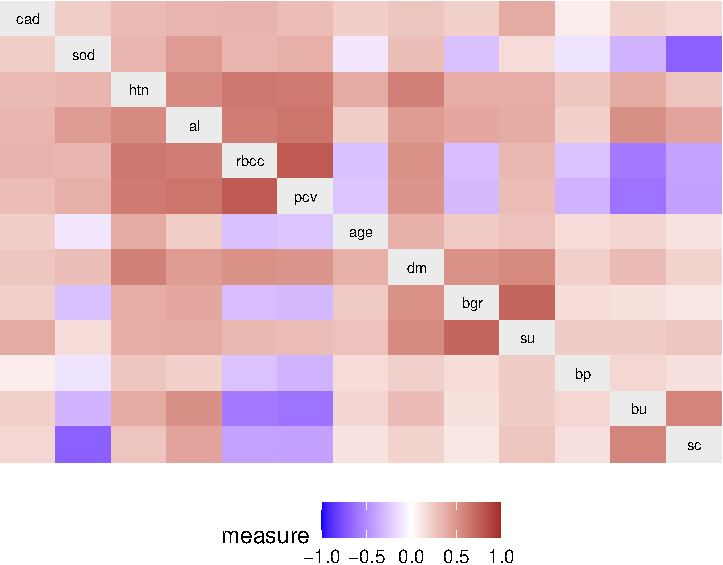
\includegraphics{rj_paper_files/figure-latex/assoc-heatmap-1} 

}

\caption[Association matrix display for penguins data showing Pearson's correlation for numeric variable pairs, canonical correlation for mixed variable pairs and categorical variable pairs]{Association matrix display for penguins data showing Pearson's correlation for numeric variable pairs, canonical correlation for mixed variable pairs and categorical variable pairs.}\label{fig:assoc-heatmap}
\end{figure}
\end{Schunk}

We can also calculate multiple association measures for all the variable
pairs in the dataset and compare them. This will help in finding out
pairs of variables with a high difference among different measures and
one can investigate these bivariate relationships in more detail. The
\texttt{pairwise\_summary\_plot} function can be used to compare various
measures using the matrix layout. It plots multiple measures among the
variable pairs as bars, where each bar represents one measure of
association. Figure \ref{fig:compare-matrix} shows a matrix layout
comparing Pearson's and Spearman's correlation coefficient for the
numeric variable pairs in \emph{penguins} data.

\begin{Schunk}
\begin{figure}

{\centering 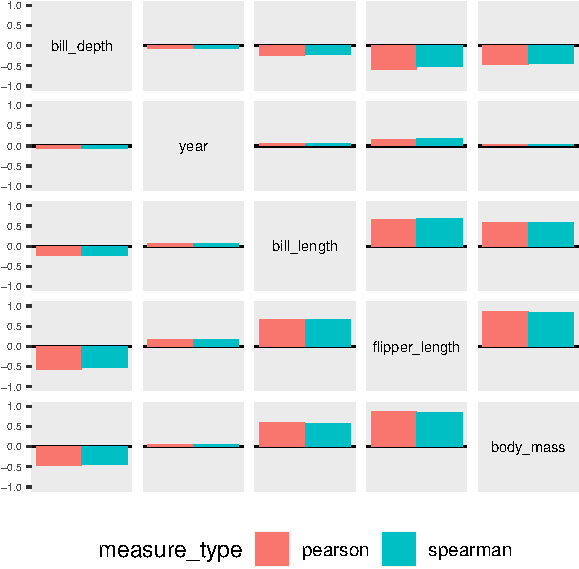
\includegraphics{rj_paper_files/figure-latex/compare-matrix-1} 

}

\caption[Matrix display comparing Pearson's and Spearman's correlation coefficient]{Matrix display comparing Pearson's and Spearman's correlation coefficient. All the variable pairs have similar values for both correlations.}\label{fig:compare-matrix}
\end{figure}
\end{Schunk}

In addition to matrix layout, we can also use linear layouts for
comparing multiple measures. Figure \ref{fig:compare-linear} shows a
linear layout comparing multiple association measures for all the
variable pairs in the penguins data. Linear layouts seems to be more
suitable when comparing high number of association measures.

\begin{Schunk}
\begin{figure}

{\centering 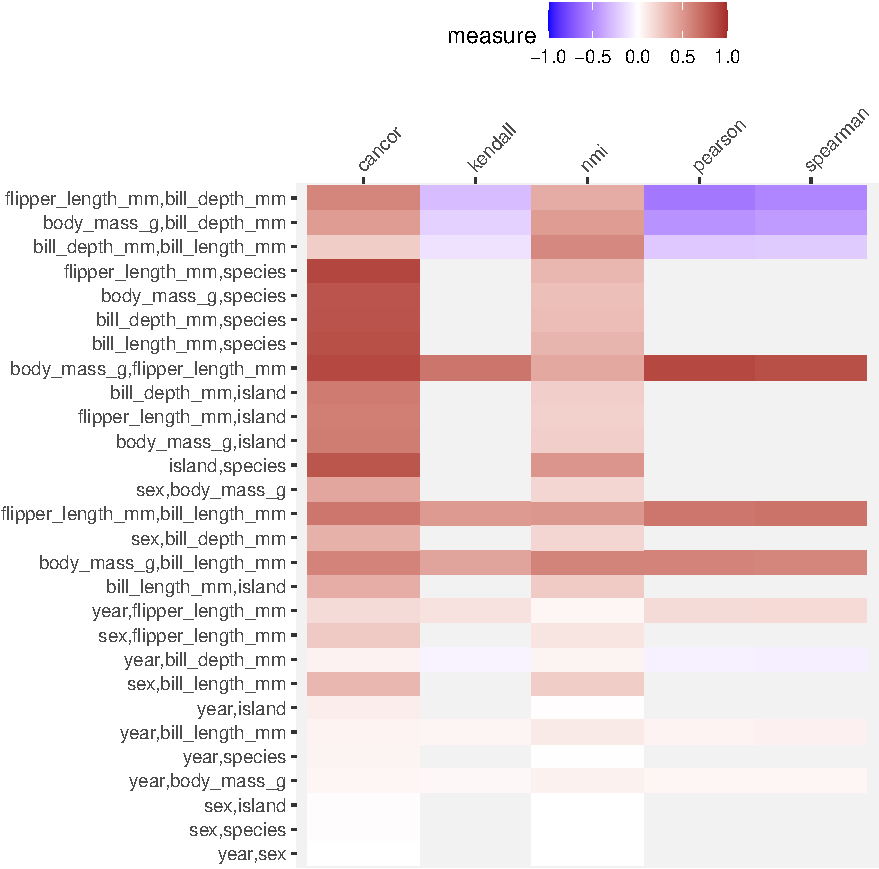
\includegraphics{rj_paper_files/figure-latex/compare-linear-1} 

}

\caption[Comparing multiple association measures using a linear layout]{Comparing multiple association measures using a linear layout. The display has variable pairs on the Y-axis and association measures on the X-axis. The cell corresponding to a variable pair and an association measure has been colored grey showing that the measure is not defined for corresponding pair.}\label{fig:compare-linear}
\end{figure}
\end{Schunk}

\hypertarget{visualising-conditional-association}{%
\subsection{Visualising Conditional
Association}\label{visualising-conditional-association}}

The package includes a function \texttt{calc\_assoc\_by} which
calculates the pairwise association at different levels of a categorical
conditioning variable. This helps in finding out interesting variable
triples which can be explored further prior to modeling. Figure
\ref{fig:cond-assoc} shows a conditional association plot for the
\emph{penguins} data. Each cell corresponding to a variable pair shows
three bars which correspond to the association measure (Pearson's
correlation for numeric pair and Normalized mutual information for other
combination of variables) calculated at the levels of conditioning
variable \emph{island}. The dashed line represents the overall
association measure. The plot shows that there is a high value for
normalised mutual information between bill\_length\_mm and species for
the penguins which lived in \emph{Biscoe} island compared to the
penguins which lived in \emph{Dream} island. It can also be seen that
the cell corresponding to variable pair flipper\_length\_mm and
bill\_depth\_mm has a high negative overall Pearson's correlation and
for the penguins which lived in \emph{Biscoe} island but positive
correlation for penguins which lived in \emph{Dream} and
\emph{Torgersen} island. This is an instance of Simpson's paradox which
can be taken into account during the modeling step.

\begin{Schunk}
\begin{figure}

{\centering 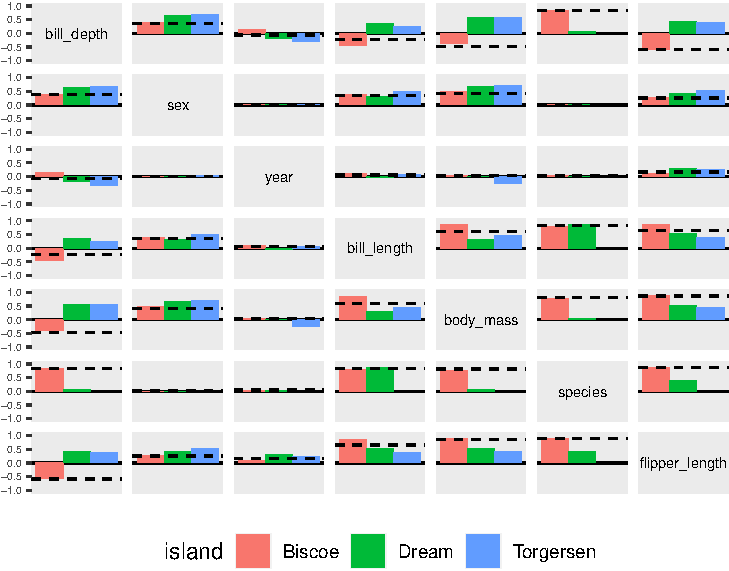
\includegraphics{rj_paper_files/figure-latex/cond-assoc-1} 

}

\caption[Conditional Association plot]{Conditional Association plot}\label{fig:cond-assoc}
\end{figure}
\end{Schunk}

We also provide a functionality for highlighting interesting patterns
like Simpson's paradox. Figure 5 shows the matrix plot with highlighted
cells for the variable pairs where Simpson's paradox is present.

\begin{Schunk}
\begin{figure}

{\centering 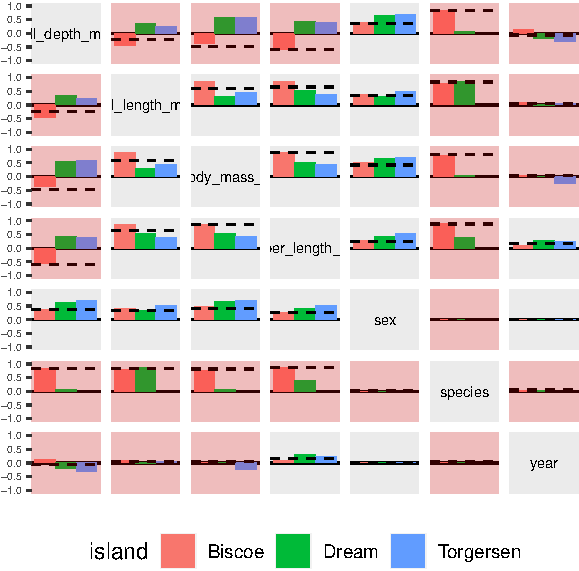
\includegraphics{rj_paper_files/figure-latex/unnamed-chunk-12-1} 

}

\caption[Conditional Association plot with Simpson's paradox]{Conditional Association plot with Simpson's paradox}\label{fig:unnamed-chunk-12}
\end{figure}
\end{Schunk}

The cells can also be highlighted on the basis of a score calculated by
the user. This can be done by providing a dataframe with pairs of
variables to highlight and a score for highlighting variable pairs. The
cells with high score will have a thicker border compared to cells with
low score. Figure 6 shows highlighted cells on the basis of a score
provided for a subset of variable pairs.

\begin{Schunk}
\begin{figure}

{\centering 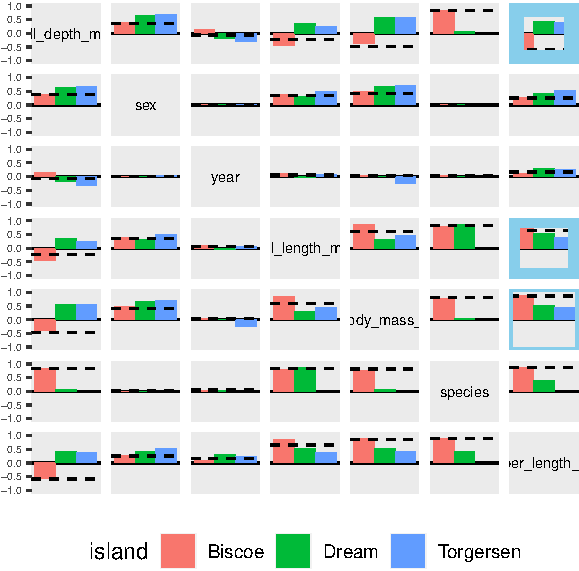
\includegraphics{rj_paper_files/figure-latex/unnamed-chunk-13-1} 

}

\caption[Conditional Association plot with manual highlighting]{Conditional Association plot with manual highlighting}\label{fig:unnamed-chunk-13}
\end{figure}
\end{Schunk}

We can also use linear layouts for displaying conditional association.
Figure 7 shows a funnel-like linear display for conditional association
measures with all the variable pairs on the y-axis, the value of
association measure on x-axis and color of the points representing the
level of the grouping variable. The linear layout becomes more useful
over the matrix layout when the number of variables and number of levels
of grouping variable are high.

\begin{Schunk}
\begin{figure}

{\centering 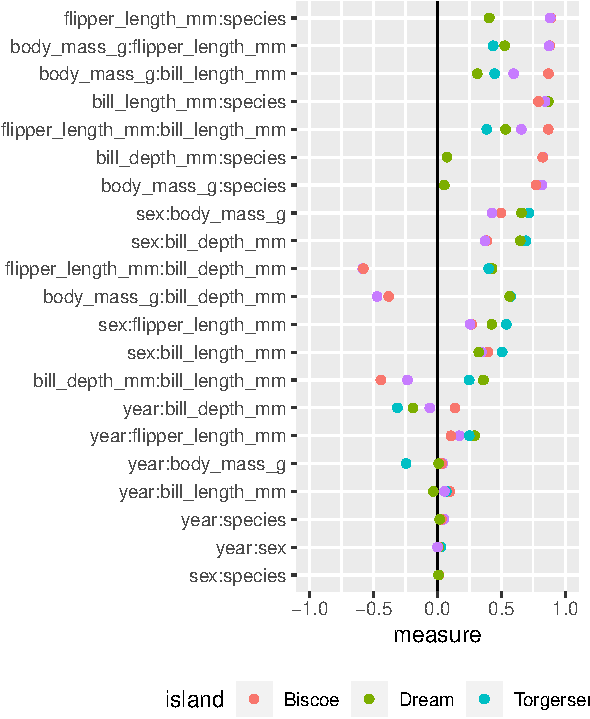
\includegraphics{rj_paper_files/figure-latex/linear_cond_assoc-1} 

}

\caption[Conditional Association plot using linear layout]{Conditional Association plot using linear layout}\label{fig:linear_cond_assoc}
\end{figure}
\end{Schunk}

\bibliography{RJreferences.bib}

\address{%
Amit Chinwan\\
Maynooth University\\%
Hamilton Institute\\ Maynooth, Ireland\\
%
%
%
\href{mailto:amit.chinwan.2019@mumail.ie}{\nolinkurl{amit.chinwan.2019@mumail.ie}}%
}

\address{%
Catherine Hurley\\
Maynooth University\\%
Department of Mathematics and Statistics\\ Maynooth, Ireland\\
%
%
%
\href{mailto:catherine.hurley@mu.ie}{\nolinkurl{catherine.hurley@mu.ie}}%
}
